\subsection{严格正函数之间的比较关系}

设 \(g\) 是 \(\mathcal{H}(\mathfrak{F},\mathbf{R})\) 中的一个函数，它在 \(\mathfrak{F}\) 的某个集上严格正。涉及 \(g\) 的比较关系可以用另一种方式表述：关系 \(\mathbf{f} \preccurlyeq g\) 等价于说 \(\| \mathbf{f}\| /g\) （它定义在 \(\mathfrak{F}\) 的某个集上）在 \(\mathfrak{F}\) 的某个集上有界；关系 \(\mathbf{f} \ll g\) 等价于说 \(\| \mathbf{f}\| /g\) 沿 \(\mathfrak{F}\) 趋于 0。若 \(f\) 是 \(\mathcal{H}(\mathfrak{F},\mathbf{R})\) 中的一个函数，则关系 \(f\asymp g\) 表示 \(f / g\) 在 \(\mathfrak{F}\) 的某个集上对数有界，而关系 \(f\sim g\) 表示 \(f / g\) 沿 \(\mathfrak{F}\) 趋于 1。若 \(f\) 是 \(\mathcal{H}(\mathfrak{F},\mathbf{R})\) 中的一个函数且在 \(\mathfrak{F}\) 的某个集上为正，则说 \(f\) 与 \(g\) 可比较蕴含 \(f / g\) 趋于一个极限（有限的或等于 \(+\infty\) ，沿 \(\mathfrak{F}\) ）。

命题 9. 设 \(f\) 与 \(g\) 是 \(\mathcal{H}(\mathfrak{F},\mathbf{R})\) 中的两个函数，在 \(\mathfrak{F}\) 的某个集上严格正。为使 \(f\) 与 \(g\) 可比较，必要且充分的是：对每个数 \(t \geqslant 0\) （至多一个例外），函数 \(f - tg\) 具有常号 \(^3\) 于 \(\mathfrak{F}\) 的某个集上。

该条件是必要的。事实上，若 \(f \ll g\) ，则有 \(f - tg \sim -tg\) （ \(t = 0\) 除外），故 \(f - tg\) 在 \(\mathfrak{F}\) 的某个集上严格负（ \(t = 0\) 除外）；若 \(f \gg g\) ，则 \(f - tg\) 在 \(\mathfrak{F}\) 的某个集上严格正（对一切 \(t\) ）；最后，若 \(f \sim kg\) （ \(k\) 为常数 \(> 0\) ），则有 \(f - tg \sim (k - t)g\) （ \(t = k\) 除外），故除 \(t = k\) 可能例外外， \(f - tg\) 具有 \(k - t\) 的符号于 \(\mathfrak{F}\) 的某个集上。

该条件是充分的。事实上，设比值 \(f / g\) 有两个不同的聚点 \(\alpha < \beta\) （沿 \(\mathfrak{F}\) ）。于是对每个数 \(t\) （满足 \(\alpha < t < \beta\) ），在每个集 \(X \in \mathfrak{F}\) 中都存在两点 \(x_{1}, x_{2}\) ，使得 \(f(x_{1}) / g(x_{1}) < t\) 且 \(f(x_{2}) / g(x_{2}) > t\) ；从而 \(f(x) - tg(x)\) 在 \(X\) 上不具有常号；我们得到了一个与假设不相容的结论。由此推出， \(f / g\) 沿以 \(\mathfrak{F}\) 为基的滤子只能有一个聚值（有限的或无穷的），从而 (Gen.~Top., I, p.~85, corollary) 沿 \(\mathfrak{F}\) 以这个值为其极限。

命题 10. 设 \(f\) 与 \(g\) 是 \(\mathcal{H}(\mathfrak{F},\mathbf{R})\) 中的两个函数，在 \(\mathfrak{F}\) 的某个集上严格正；对每个实数 \(\alpha\) 且 \(\neq 0\) ，关系 \(f\asymp g\) （相应地， \(f\sim g\) ）等价于 \(f^{\alpha}\asymp g^{\alpha}\) （相应地， \(f^{\alpha}\sim g^{\alpha}\) ）；若 \(\alpha >0\) ，关系 \(f\preccurlyeq g\) （相应地， \(f\ll g\) ）等价于 \(f^{\alpha}\preccurlyeq g^{\alpha}\) （相应地， \(f^{\alpha}\ll g^{\alpha}\) ）；若 \(\alpha < 0\) ，它等价于 \(f^{\alpha}\succcurlyeq g^{\alpha}\) （相应地， \(f^{\alpha}\gg g^{\alpha}\) ）。

证明都是直接的。

我们注意到，在 \(\mathcal{H}(\mathfrak{F},\mathbf{R})\) 中，在 F 的某个集上严格正的函数所成的集 \(\varGamma\) 使得 \(\varGamma/\mathrm{R}_{\infty}\) 是一个乘法群 \(\varGamma_{\infty}\) （在 \(\mathcal{H}_{\infty}(\mathfrak{F},\mathbf{R})\) 中）； \(\varGamma/\mathrm{R}_{0}\) 恒同于 \(\varGamma_{\infty}\) 关于（模 \(R_{\infty}\) ） \(\varGamma\) 中对数有界函数的类所成的子群的商群；在 \(\varGamma/R_{0}\) 上，由关系 \(f \preccurlyeq g\) 通过过渡到商而导出的序关系与 \(\varGamma/R_{0}\) 的群结构相容，从而使之成为一个有序群。

命题 11. 设 g 是 \(\mathcal{H}(\mathfrak{F},\mathbf{R})\) 中的一个函数，使得 \(\lim_{\mathfrak{F}}g = +\infty\) ；则关系 \(f \ll g\) 蕴含 \(e^{f} \ll e^{g}\) ；关系 \(f \sim g\) 蕴含 \(\log f \sim \log g\) 。

事实上，若 \(f \ll g\) ，则 \(f - g = g\left(\frac{f}{g} - 1\right)\) 趋于 \(-\infty\) （沿 \(\mathfrak{F}\) ）。类似地，若 \(f \sim g\) ，则有 \(\log f = \log g + \log \frac{f}{g}\) ，故 \(\log f - \log g\) 趋于 0，对 \(\frac{\log f}{\log g} - 1 = \frac{\log f - \log g}{\log g}\) 亦然。

\pandocbounded{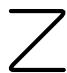
\includegraphics[keepaspectratio]{images/part002_2162bedd.jpg}}

另一方面，注意关系 \(f \sim g\) 并不蕴含 \(e^{f} \sim e^{g}\) ，甚至不蕴含 \(e^{f} \asymp e^{g}\) ，正如例子 \(f(x) = x^{2}\) 、 \(g(x) = x^{2} + x\) （当 x 趋于 \(+\infty\) 时）所表明的；类似地，关系 \(f \ll g\) 并不蕴含 \(\log f \ll \log g\) ，正如例子 \(f(x) = x\) 、 \(g(x) = x^{2}\) （当 x 趋于 \(+\infty\) 时）所表明的。

定义 5. 设 g 是 \(\mathcal{H}(\mathfrak{F},\mathbf{R})\) 中的一个函数，在 F 的某个集上严格正，且使得 \(\lim_{\mathfrak{F}}g=0\) 或 \(\lim_{\mathfrak{F}}g=+\infty\) 。我们说函数 \(f\in\mathcal{H}(\mathfrak{F},\mathbf{R})\) 相对于 g 是 \(\rho\) 阶的（有限或无穷），如果 \(\lim_{\mathfrak{F}}\log(|f|)/\log g=\rho\) 。

注意，若 f 相对于 g 是 \(\rho\) 阶的，则 f 相对于 1/g 是 \(-\rho\) 阶的；因此只需处理 \(g(x)\) 沿 F 趋于 \(+\infty\) 的情形。

\pandocbounded{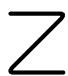
\includegraphics[keepaspectratio]{images/part002_5139c9a2.jpg}}

命题 12. 设 \(g\) 是 \(\mathcal{H}(\mathfrak{F},\mathbf{R})\) 中的一个函数，使得 \(\lim_{\mathfrak{F}}g = +\infty\) ；设 \(f\) 是 \(\mathcal{H}(\mathfrak{F},\mathbf{R})\) 中的一个函数。

\begin{enumerate}
\def\labelenumi{\alph{enumi})}
\item
  为使 \(f\) 是 \(+\infty\) 阶的（相对于 \(g\) ），必要且充分的是 \(f \gg g^{\alpha}\) （对每个 \(\alpha \geqslant 0\) ）。
\item
  为使 \(f\) 是 \(-\infty\) 阶的（相对于 \(g\) ），必要且充分的是 \(f \ll g^{-\alpha}\) （对每个 \(\alpha > 0\) ）。
\item
  为使 \(f\) 是等于 \(\rho\) 的有限阶（相对于 \(g\) ），必要且充分的是：对每个 \(\varepsilon > 0\) ，有 \(g^{\rho - \varepsilon} \ll f \ll g^{\rho + \varepsilon}\) 。
\end{enumerate}

例如我们证明 c)。若 \(f\) 相对于 \(g\) 的阶是 \(\rho\) ，则对每个 \(\varepsilon > 0\) ，存在一个集 \(\mathbf{M} \in \mathfrak{F}\) ，使得对每个 \(x \in \mathbf{M}\) ，我们有

\[
\left(\rho - \frac {\varepsilon}{2}\right) \log g (x) \leqslant \log | f (x) | \leqslant \left(\rho + \frac {\varepsilon}{2}\right) \log g (x),
\]

或者 \((g(x))^{\rho-\frac{\varepsilon}{2}} \leqslant |f(x)| \leqslant (g(x))^{\rho+\frac{\varepsilon}{2}}\) ；由于 \(\lim_{\mathfrak{F}} g = +\infty\) ，于是有 \(g^{\rho-\varepsilon} \ll f \ll g^{\rho+\varepsilon}\) （对每个 \(\varepsilon > 0\) ）；其逆是直接的。a) 与 b) 的证明类似。

注意，若 \(f\) 是有限阶 \(\rho\) （相对于 \(g\) ），则 \(fg^{-\rho}\) 相对于 \(g\) 是 0 阶，反之亦然；若 \(f_1\) （相应地， \(f_2\) ）是 \(\rho_1\) 阶（相应地， \(\rho_2\) 阶）的（相对于 \(g\) ），且 \(\rho_1 + \rho_2\) 有定义，则 \(f_1f_2\) 是 \(\rho_1 + \rho_2\) 阶的（相对于 \(g\) ）。

注. 1) 注意，尽管 f 相对于 g 可以是有限阶 \(\rho\) ，但比值 \(f/g^{\rho}\) 未必趋于一个极限；例如，每个对数有界函数相对于 g 都是 0 阶的，但沿 F 未必有极限。

\begin{enumerate}
\def\labelenumi{\arabic{enumi})}
\setcounter{enumi}{1}
\tightlist
\item
  一个定义在 \(\mathfrak{F}\) 的某个集上的函数未必相对于 \(g\) 有确定的阶（有限的或否），因为相对于 \(g\) 有确定阶的函数与 \(g\) 的一切幂可比较（至多一个例外）。而 \(f\) 未必具有这个性质，例子 \(g(x) = x\) 、 \(f(x) = 1 + x^2 \sin^2 x\) （当 \(x\) 趋于 \(+\infty\) 时）便表明了这一点。在这个例子中， \(f\) 与 \(g^\alpha\) 可比较（对 \(\alpha < 0\) 与 \(\alpha > 2\) ）；若取 \(f(x) = e^x \sin^2 x + e^{-x} \cos^2 x\) ，则 \(f\) 不与 \(g\) 的任何幂（正的或负的）可比较。
\end{enumerate}

